% F0 — the hero schematic for Spectral Surface Generation.
% One quantum measurement (the overlap bank, paid once) -> the whole (lambda,tau)
% spectral surface and every diagnostic, by classical post-processing.
% Thesis: quantum resources maximised classically.
\documentclass[tikz,border=4pt]{standalone}
\usepackage{amsmath}
\usepackage{bm}
\usetikzlibrary{arrows.meta,positioning,backgrounds,fit,calc}

\definecolor{ink}{HTML}{1A1A2E}
\definecolor{phys}{HTML}{2C6FAD}
\definecolor{acc}{HTML}{C0392B}
\definecolor{faint}{HTML}{9AA5B1}
\definecolor{physbg}{HTML}{EAF1F8}
\definecolor{inkbg}{HTML}{F2F3F5}

\begin{document}
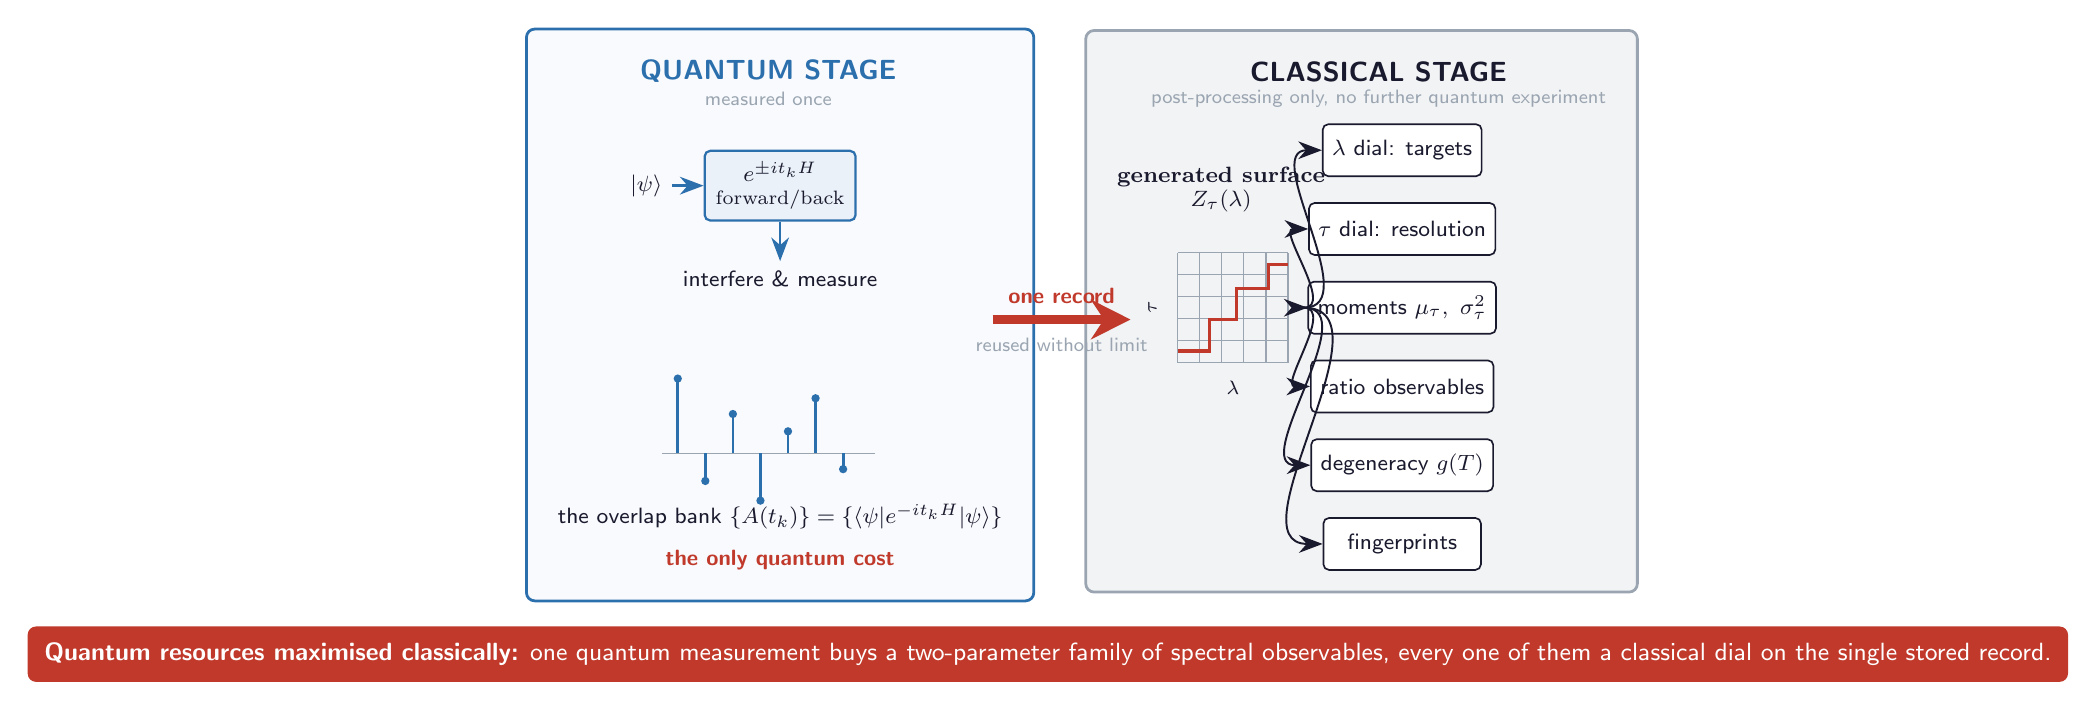
\begin{tikzpicture}[
  font=\sffamily,
  >={Stealth[length=3mm]},
  stage/.style={rounded corners=3pt, line width=1pt, inner sep=8pt},
  dial/.style={rounded corners=2pt, draw=ink, line width=0.6pt, fill=white,
               inner sep=3.4pt, font=\footnotesize\sffamily, text=ink,
               minimum height=6.6mm, minimum width=20mm, align=center},
  lab/.style={font=\footnotesize\sffamily, text=ink},
]

% ============================ QUANTUM STAGE (left) ==========================
\begin{scope}[local bounding box=Q]
  \node[lab, text=phys, font=\bfseries\sffamily] (qh) at (0,3.35) {QUANTUM STAGE};
  \node[lab, text=faint, font=\scriptsize\sffamily] at (0,3.0) {measured once};

  \node[lab, text=ink] (psi) at (-1.55,1.9) {$|\psi\rangle$};
  \node[draw=phys, line width=0.8pt, rounded corners=2pt, fill=physbg,
        inner sep=4pt, font=\footnotesize, text=ink, align=center] (ev)
        at (0.15,1.9) {$e^{\pm i t_k H}$\\[-1pt]{\scriptsize forward/back}};
  \draw[->, phys, line width=0.9pt] (psi) -- (ev);
  \node[lab, text=ink, align=center] (meas) at (0.15,0.72)
       {\footnotesize interfere \& measure};
  \draw[->, phys, line width=0.9pt] (ev) -- (meas);

  \begin{scope}[shift={(-1.35,-1.5)}]
    \draw[faint, line width=0.5pt] (0,0) -- (2.7,0);
    \foreach \x/\h in {0.2/0.95,0.55/-0.35,0.9/0.5,1.25/-0.6,1.6/0.28,1.95/0.7,2.3/-0.2}{
      \draw[phys, line width=1pt] (\x,0) -- (\x,\h);
      \fill[phys] (\x,\h) circle (1.5pt);
    }
  \end{scope}
  \node[lab, text=ink] at (0.15,-2.3)
       {the overlap bank $\{A(t_k)\}=\{\langle\psi|e^{-it_kH}|\psi\rangle\}$};
  \node[lab, text=acc, font=\footnotesize\bfseries\sffamily] at (0.15,-2.85)
       {the only quantum cost};
\end{scope}
\begin{scope}[on background layer]
  \node[stage, draw=phys, fill=physbg!35, fit=(Q)] {};
\end{scope}

% ============================ REUSE ARROW (center) ==========================
\draw[-{Stealth[length=5mm,width=5mm]}, acc, line width=3pt]
      (2.85,0.2) -- node[above=1pt, font=\footnotesize\bfseries\sffamily, text=acc]{one record}
                    node[below=2pt, font=\scriptsize\sffamily, text=faint]{reused without limit}
      (4.6,0.2);

% ========================== CLASSICAL STAGE (right) =========================
\begin{scope}[local bounding box=C, shift={(5.05,0)}]
  \node[lab, text=ink, font=\bfseries\sffamily] (ch) at (2.7,3.35) {CLASSICAL STAGE};
  \node[lab, text=faint, font=\scriptsize\sffamily] at (2.7,3.0)
       {post-processing only, no further quantum experiment};

  % the generated surface Z_tau(lambda): a little (lambda,tau) grid with a staircase
  \begin{scope}[shift={(0.15,-0.35)}]
    \foreach \i in {0,...,5}{ \draw[faint, line width=0.4pt] (\i*0.28,0) -- (\i*0.28,1.4); }
    \foreach \j in {0,...,5}{ \draw[faint, line width=0.4pt] (0,\j*0.28) -- (1.4,\j*0.28); }
    \draw[acc, line width=1.1pt] (0,0.15) -- (0.4,0.15) -- (0.4,0.55) -- (0.75,0.55)
          -- (0.75,0.95) -- (1.15,0.95) -- (1.15,1.25) -- (1.4,1.25);
    \node[lab, text=ink, font=\scriptsize] at (0.7,-0.32) {$\lambda$};
    \node[lab, text=ink, font=\scriptsize, rotate=90] at (-0.32,0.7) {$\tau$};
  \end{scope}
  \node[lab, text=ink, font=\footnotesize\bfseries, align=center] at (0.7,1.85)
       {generated surface\\[-1pt]$Z_\tau(\lambda)$};

  % the fan of classical dials/readouts
  \node[dial] (d1) at (3.0,2.35) {$\lambda$ dial: targets};
  \node[dial] (d2) at (3.0,1.35) {$\tau$ dial: resolution};
  \node[dial] (d3) at (3.0,0.35) {moments $\mu_\tau,\ \sigma^2_\tau$};
  \node[dial] (d4) at (3.0,-0.65) {ratio observables};
  \node[dial] (d5) at (3.0,-1.65) {degeneracy $g(T)$};
  \node[dial] (d6) at (3.0,-2.65) {fingerprints};
  \foreach \d in {d1,d2,d3,d4,d5,d6}{
    \draw[->, ink, line width=0.7pt] (1.75,0.35) to[out=0,in=180] (\d.west);
  }
\end{scope}
\begin{scope}[on background layer]
  \node[stage, draw=faint, fill=inkbg, fit=(C)] {};
\end{scope}

% ============================ THE THESIS (bottom) ===========================
\node[rounded corners=3pt, fill=acc, text=white, font=\small\sffamily,
      inner sep=6pt, align=center, minimum width=200mm]
      at (3.55,-4.05)
      {\textbf{Quantum resources maximised classically:} one quantum measurement
       buys a two-parameter family of spectral observables, every one of them a
       classical dial on the single stored record.};

\end{tikzpicture}
\end{document}
